\input{shortcuts}

\section{CP Violation in  $B$ mesons}
\label{sec:cpv}
Since its discovery in the kaon system, CP violation has been an intriguing field. A lot of efforts have been put in understanding it, as,  a part from the interest of the phenomenon by itself and of its relations with the matter/antimatter asymmetry, it is a very powerful probe for NP.  In fact,  CP violation is particularly interesting because, in the SM, it originates from a single parameter. All the CP violating observables in the $K$, $D$ and $B$ meson sectors are thus directly related and
their combined study provides a highly powerful test of the whole SM dynamics.
Instead, most model of New Physics are far less restrictive and allow for a
plethora of new CP-violating sources. None of the delicate interplays between
observables expected in the SM should survive to the presence of new dynamics
at the~TeV scale.


When experimentally testing SM predictions, it is fundamental that the
theoretical precision matches the experimental accuracy. A priori, this looks
challenging because CP-violation is a purely hadronic phenomenon in the SM,
originating from the quark couplings. However, dedicated strategies have been
designed and CP-violating observables are actually among our best windows to look through when searching for  NP. For
example, in CP-violating asymmetries, most of the uncertainties cancel between
the numerator and the denominator, so that we can construct measurable
quantities with small uncertainties. Alternatively, some observables are
predicted to be so small that they can be considered forbidden in the SM, and
simply observing a non-zero value would unequivocally signal the presence of
New Physics.

The French community has been deeply involved in CP-violation dedicated experiments for
many years (CPLEAR, NA48, BaBar, LHCb). It has been designing, building and maintaining key
elements of the detectors, like trigger and calorimeters. Expertise has been developed in
several key techniques needed to study CP-violation: amplitude analyses, tagged-time-dependent
angular analyses, flavour tagging, neutral objects reconstruction. From the analysis point of view,   the
French community has been involved more specifically in the measurements of the Unitarity angles
$\alpha$, $\gamma$ and $\phi_{s}$. Among other decay channels, the following
have been
studied in detail:
$B_{(s,d)}\to D^{0} K^{*0}$, $B_{(s,d)}\to\bar{D}^{0} hh$, $B^{0}_{s} \to
D_{s} K$, $B^{0}_{s} \to J/\psi\phi$,
$B^{0}_{s} \to J/\psi\bar{K}^{*0}$. 
One of the outcome of the work done is
$\phi_{s}$ is illustrated on Figure~\ref{figphis}.  
% $B^{0}\to\rho\rho$, $B_{(s,d)}\to K^{0}_{\mathrm{S}} hh$, $B^{0} \to K^{0}_{\mathrm{S}} K \pi$,

CP-violation related studies of charmless $b$-hadron decays are another field in which the experimental French groups have been  very active in the B-factories era, and still are nowadays.  These decays have a number of theoretical applications and provide a probe to new physics. For instance, the decays \BdtoKsPiPi and \BdtoKsKK are dominated by \btoqqbars ($q = u,d,s$) loop transitions.  Mixing-induced \CP asymmetries in such decays are predicted to be approximately equal to those in \btoccbars transitions, \eg $\Bd\to\jpsi\KS$, by the
Cabibbo-Kobayashi-Maskawa mechanism~\cite{Cabibbo:1963yz,Kobayashi:1973fv}.
However, the loop diagrams that dominate the charmless decays can have
contributions from new particles in several extensions of the Standard Model,
which could introduce additional weak phases~\cite{Buchalla:2005us,Grossman:1996ke,London:1997zk,Ciuchini:1997zp}.
A time-dependent analysis of the three-body Dalitz plot allows measurements of
the mixing-induced \CP-violating
phase~\cite{Dalseno:2008wwa,Aubert:2009me,Nakahama:2010nj,Lees:2012kxa}. 
 The current experimental measurements of \btoqqbars decays~\cite{HFAG} show
fair agreement with the results from \btoccbars decays (measuring the weak
phase \Pbeta) for each of the scrutinised \CP eigenstates.
There is, however, a global trend towards lower values than the weak phase
measured from \btoccbars decays.
The interpretation of this deviation is made complicated by QCD
corrections, which depend on the final state~\cite{Silvestrini:2007yf} and
are difficult to handle.
An analogous extraction of the mixing-induced \CP-violating phase in the
\Bs system ($\beta_s$) will, with a sufficiently large dataset, also be possible with
the \BstoKsKPi decay, which can be compared with that from, \eg
$\Bs\to\jpsi\phi$.

The charmless three-body analyses provide a long-term physics programs that can profit from the LHCb upgrade. In fact, these analyses proceed in increasingly complex steps, which become more and more sensitive to new physics observables with the growing dataset, and with more observed decay modes. One of the long-term goals is to perform full flavor- and time-dependent Dalitz-plot analyses of the \BstoKshhp modes to measure the weak phases $\beta$ and $\beta_s$. Recent theoretical and experimental activity has focused on the determination of the CKM angle \Pgamma from charmless $B$ meson decays using and refining the methods proposed in Refs.~\cite{Ciuchini:2006kv,Gronau:2006qn,Bhattacharya:2013cla}. Moreover, with the upgrade of LHCb, more modes, eventually with more neutral hadrons, are being considered. 




%+ PCI40, SciFi
%CPLEAR, NA48, NA62, BaBar, LEP(?) LHCb

In the coming years, most of the experimental effort will go into the analysis of data collected by  LHCb during run2 and in its
upgrade plans. 

%One of the biggest challenge will be to store and analyse the enormous quantity of data from the LHC.

%CHRISTOPHER>
From the theory side, ... CKMfitter, QCD challenge, precision challenge,
sub-leading diagram estimation, penguin pollution, ...

In the next five years, the GDR   will provide the opportunity to continue the
measurements started many years ago using the full run2 dataset of the LHC,
and to explore new routes. In summary:

\begin{itemize}
\item the effort on the measurement of $\phi_{s}$ will continue, with a focus on controlling the sub-leading penguins contributions;
\item several ways to measure $\gamma$ and $\alpha$ will be explored, using for example charmless $B$ decays;
\item CP violation in baryons, largely produced at the LHC  is currently a mostly unexplored field, complementary to the meson field, that we will have the opportunity to explore;
\item CP violation in charm,  still to be discovered, will be searched for;
\item the theoretical advancement in CP violation in kaon, like  lattice studies of the $\varepsilon^{\prime}$ matrix elements, will be followed, together with the achievements of the  NA62 experiment, currently in data taking and aiming to mesure the  $K^{+}%
\rightarrow\pi^{+}\nu\nu$ branching fraction.
\item EDM: should we include the nEDM experiment? It is among the IN2P3 projects.
\end{itemize}

For all these items, the synergy between experimental and theoretical communities is essential, because a major discovery can not come if the uncertainties are not under control in both places. The new data coming from the LHC and soon from Belle2, as well as from NA62 will certainly allow to make important advancements in the CP violation field, and we need to ensure to provide our contribution and to correctly interpret the measurements in the global CP violation picture. 

%It should be noted that there is a clear interplay of this working group with the We will also actively participate to the brainstorming on future upgrade of the LHCb experiment, i.e. plans for the 2025-2035 period.

\begin{figure}[!htb]
\begin{center}
\includegraphics[width=7.5cm]{hfag_Spring2016_DGsphis_zoom.pdf}
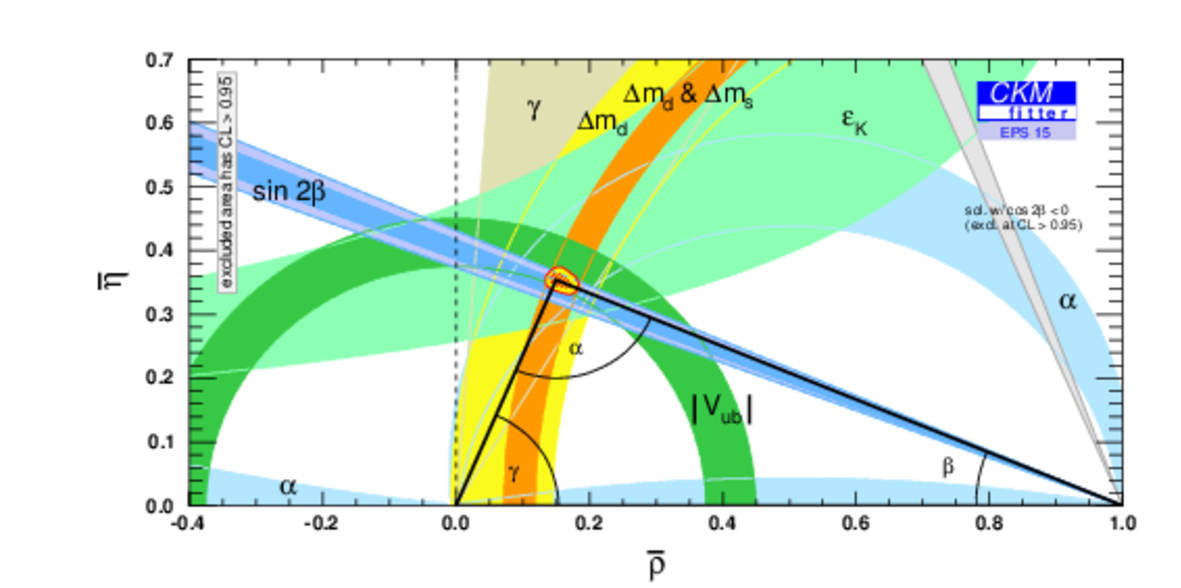
\includegraphics[width=7.5cm]{rhoeta_small_global.pdf}
\end{center}
\caption{Left plot: 68\% CL regions in $B^{0}_{s}$ width difference $\Delta\Gamma_{s}$
and weak phase $\phi_{s}$ obtained from individual and combined CDF, D0,
ATLAS, CMS and LHCb likelihoods of $B^{0}_{s}\to J/\psi\phi$, $B^{0}_{s}\to
J/\psi KK$, $B^{0}_{s}\to J\psi\pi\pi$ and $B^{0}_{s}\to D_{s}^{+}D_{s}^{-}%
$.The expectation within the Standard Model is shown as the black rectangle. Right plot: the current status of the CKM unitarity triangle test from the CKMFitter collaboration. }%
\label{figphis}%
\end{figure}




%
%\section{Charmless $b$ Hadron Decays}
%\label{sec:charmless}
%
%The study of of $b$-hadron decays to hadronic final states with no charmed particles allow for a rich array of studies. A few examples are the measurements of branching fractions, CP asymmetries, weak and strong phases and the CKM angles; they probe the dynamics of weak and strong interactions. The typical branching fractions of these modes are below $10^{-5}$ and thus their analyses are feasible only with large data samples and the use of powerful tools to reject background. The LHCb experiment is an adequate experimental environment for these analyses, offering the possibility to study decays of light $B$ mesons, $B_s$ mesons and $b$ baryons.
%
%In particular, CP-violation related studies of charmless $b$-hadron decays have a number of theoretical applications and that provide a probe to new physics, along the lines described in Sec.~\ref{sec:cpv}.
%For instance, the decays \BdtoKsPiPi and \BdtoKsKK are dominated by \btoqqbars ($q = u,d,s$)
%loop transitions.
%Mixing-induced \CP asymmetries in such decays are predicted to be approximately
%equal to those in \btoccbars transitions, \eg $\Bd\to\jpsi\KS$, by the
%Cabibbo-Kobayashi-Maskawa mechanism~\cite{Cabibbo:1963yz,Kobayashi:1973fv}.
%However, the loop diagrams that dominate the charmless decays can have
%contributions from new particles in several extensions of the Standard Model,
%which could introduce additional weak phases~\cite{Buchalla:2005us,Grossman:1996ke,London:1997zk,Ciuchini:1997zp}.
%A time-dependent analysis of the three-body Dalitz plot allows measurements of
%the mixing-induced \CP-violating
%phase~\cite{Dalseno:2008wwa,Aubert:2009me,Nakahama:2010nj,Lees:2012kxa}. 
% The current experimental measurements of \btoqqbars decays~\cite{HFAG} show
%fair agreement with the results from \btoccbars decays (measuring the weak
%phase \Pbeta) for each of the scrutinised \CP eigenstates.
%There is, however, a global trend towards lower values than the weak phase
%measured from \btoccbars decays.
%The interpretation of this deviation is made complicated by QCD
%corrections, which depend on the final state~\cite{Silvestrini:2007yf} and
%are difficult to handle.
%An analogous extraction of the mixing-induced \CP-violating phase in the
%\Bs system ($\beta_s$) will, with a sufficiently large dataset, also be possible with
%the \BstoKsKPi decay, which can be compared with that from, \eg
%$\Bs\to\jpsi\phi$.
%
%An impressive harvest of results from charmless hadronic $B$ mesons decays was obtained by the $B$ factories. Several french groups participated in these studies within the BaBar experiment, and in particular, a part of the present LPNHE-LHCb group. The LHCb experiment is already playing an important role in this area of physics, with the participation of the LPC and LPNHE groups. Both have contributed to the LHCb analysis of the decay modes \BstoKshhp ($\had^{(\prime)} = \pi, K$) with $1$~fb$^{-1}$ of data, which are being pursued with $3$~fb$^{-1}$.  In particular they are performing amplitude analyses (aka Dalitz-plot analyses) of \BdtoKsPiPi and \BdtoKsKK decays. At LHCb, the first step of the charmless $b$ hadron decays physics programme is to establish the signals of yet unobserved rare modes. The only yet-unobserved \BstoKshhp mode is \BstoKsKK. The LPC group also performs analyses of $B_s \to \rho^0 \rho^0$, and $\Lambda_b^0 (\Xi_b^0) \to p \had \had^{\prime}\had^{\prime\prime}$ decays.
%
%All the analyses mentioned above provide a long-term physics programs that can profit from the LHCb upgrade. These analyses proceed in increasingly complex steps, which become more and more sensitive to new physics observables with the growing dataset, and with more observed decay modes. One of the long-term goals is to perform full flavor- and time-dependent Dalitz-plot analyses of the \BstoKshhp modes to the measure the weak phases $\beta$ and $\beta_s$. Recent theoretical and experimental activity has focused on the determination of the CKM angle \Pgamma from charmless $B$ meson decays using and refining the methods proposed in Refs.~\cite{Ciuchini:2006kv,Gronau:2006qn,Bhattacharya:2013cla}. The LPNHE group is checking the applicability of the method described in the last reference to the LHCb physics analysis. Moreover, with the upgrade of LHCb, more modes, eventually with more neutral hadrons, are being considered.